%%%%%%%%%%%%%%%%%%%%%%%%%%%%%%%%%%%%%%%%%
% Jacobs Landscape Poster
% LaTeX Template
% Version 1.0 (29/03/13)
%
% Created by:
% Computational Physics and Biophysics Group, Jacobs University
% https://teamwork.jacobs-university.de:8443/confluence/display/CoPandBiG/LaTeX+Poster
% 
% Further modified by:
% Nathaniel Johnston (nathaniel@njohnston.ca)
%
% This template has been downloaded from:
% http://www.LaTeXTemplates.com
%
% License:
% CC BY-NC-SA 3.0 (http://creativecommons.org/licenses/by-nc-sa/3.0/)
%
%%%%%%%%%%%%%%%%%%%%%%%%%%%%%%%%%%%%%%%%%

%----------------------------------------------------------------------------------------
%	PACKAGES AND OTHER DOCUMENT CONFIGURATIONS
%----------------------------------------------------------------------------------------

\documentclass[final]{beamer}

\usepackage[scale=1.24]{beamerposter} % Use the beamerposter package for laying out the poster

\usetheme{confposter} % Use the confposter theme supplied with this template

\setbeamercolor{block title}{fg=ngreen,bg=white} % Colors of the block titles
\setbeamercolor{block body}{fg=black,bg=white} % Colors of the body of blocks
\setbeamercolor{block alerted title}{fg=white,bg=dblue!70} % Colors of the highlighted block titles
\setbeamercolor{block alerted body}{fg=black,bg=dblue!10} % Colors of the body of highlighted blocks
% Many more colors are available for use in beamerthemeconfposter.sty

%-----------------------------------------------------------
% Define the column widths and overall poster size
% To set effective sepwid, onecolwid and twocolwid values, first choose how many columns you want and how much separation you want between columns
% In this template, the separation width chosen is 0.024 of the paper width and a 4-column layout
% onecolwid should therefore be (1-(# of columns+1)*sepwid)/# of columns e.g. (1-(4+1)*0.024)/4 = 0.22
% Set twocolwid to be (2*onecolwid)+sepwid = 0.464
% Set threecolwid to be (3*onecolwid)+2*sepwid = 0.708

\newlength{\sepwid}
\newlength{\onecolwid}
\newlength{\twocolwid}
\newlength{\threecolwid}
\setlength{\paperwidth}{48in} % A0 width: 46.8in
\setlength{\paperheight}{36in} % A0 height: 33.1in
\setlength{\sepwid}{0.024\paperwidth} % Separation width (white space) between columns
\setlength{\onecolwid}{0.22\paperwidth} % Width of one column
\setlength{\twocolwid}{0.464\paperwidth} % Width of two columns
\setlength{\threecolwid}{0.708\paperwidth} % Width of three columns
\setlength{\topmargin}{-0.5in} % Reduce the top margin size
%-----------------------------------------------------------

\usepackage{graphicx}  % Required for including images

\usepackage{booktabs} % Top and bottom rules for tables

%----------------------------------------------------------------------------------------
%	TITLE SECTION 
%----------------------------------------------------------------------------------------

\title{Visualize 3D scientific data in a Pythonic way like matplotlib} % Poster title

\author{Tetsuo Koyama} % Author(s)

\institute{PyVista developers team} % Institution(s)

%----------------------------------------------------------------------------------------

\begin{document}

\addtobeamertemplate{block end}{}{\vspace*{2ex}} % White space under blocks
\addtobeamertemplate{block alerted end}{}{\vspace*{2ex}} % White space under highlighted (alert) blocks

\setlength{\belowcaptionskip}{2ex} % White space under figures
\setlength\belowdisplayshortskip{2ex} % White space under equations

\begin{frame}[t] % The whole poster is enclosed in one beamer frame

\begin{columns}[t] % The whole poster consists of three major columns, the second of which is split into two columns twice - the [t] option aligns each column's content to the top

\begin{column}{\sepwid}\end{column} % Empty spacer column

\begin{column}{\onecolwid} % The first column

%----------------------------------------------------------------------------------------
%	OBJECTIVES
%----------------------------------------------------------------------------------------

\begin{alertblock}{Abstract}

Using WebRTC we are trying to develop a product called 'Ping' used for audio, mult-video, file and screen sharing.
\begin{itemize}
\item Ping uses WebRTC for the source of data exchange and XMPP Server for signalling and transporting.
\item Ping works on Browser to Browser connections instead of naive client server approach.
\item Ping guarentees high scalability and upto 60\% more efficiency than existing systems.
\end{itemize}

\end{alertblock}

%----------------------------------------------------------------------------------------
%	INTRODUCTION
%----------------------------------------------------------------------------------------

\begin{block}{Introduction}

\begin{itemize}
\item WebRTC is an upcoming standard that aims to improve real time communication among web browsers in peer to peer fashion.
\item Ping uses WebRTC which allows browsers to natively support interactive peer to peer communication and realtime collaboration.
\item Ping is a low cost highly efficient solution for data communication.
\item Ping improves the state of audio/video communication stack in the browser
\item Ping leverages the specification to achieve interoperability among web browsers.
\item Unlike existing systems, Ping doesn't require any plugins, extensions and signups. 
\end{itemize}



\end{block}

%------------------------------------------------

\begin{figure}
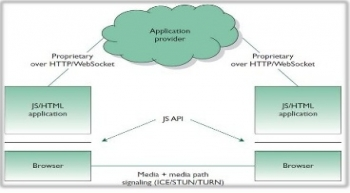
\includegraphics[width=0.8\linewidth]{step0002.jpg}
\caption{Architecture of Ping}
\end{figure}

%----------------------------------------------------------------------------------------

\end{column} % End of the first column

\begin{column}{\sepwid}\end{column} % Empty spacer column

\begin{column}{\twocolwid} % Begin a column which is two columns wide (column 2)

\begin{columns}[t,totalwidth=\twocolwid] % Split up the two columns wide column

\begin{column}{\onecolwid}\vspace{-.6in} % The first column within column 2 (column 2.1)

%----------------------------------------------------------------------------------------
%	MATERIALS
%----------------------------------------------------------------------------------------

\begin{block}{Architecture}

We designed an efficient architecture for Ping to withstand high traffic.

\begin{itemize}
\item At start browsers do not know each other.
\item WebRTC mediates the setup process through the XMPP server of Ping.
\item All browsers connected to a particular media object are called to be a part of a swarm and are assigned unique id's.
\item Browsers speak to other browsers in the swarm.
\item Media flows through the shortest possible path for latency.
\item An XMPP server in the backend is used for signalling and initial connection.
\end{itemize}



\end{block}

%----------------------------------------------------------------------------------------

\end{column} % End of column 2.1

\begin{column}{\onecolwid}\vspace{-.6in} % The second column within column 2 (column 2.2)

%----------------------------------------------------------------------------------------
%	METHODS
%----------------------------------------------------------------------------------------

\begin{block}{Security}

\begin{itemize}
\item Ping is resistant to several security problems.
\item Ping implementations use secure protocols such as DTLS and SRTP.
\item Encryption is mandatory for all Ping components including signaling mechanism.
\item Ping runs in a browser sandbox and is not a separate process. 
\item Ping doesn't require separate plugins or components.
\item Hashes of the end objects are compared to find any packet loss.
\end{itemize}

\end{block}

%----------------------------------------------------------------------------------------

\end{column} % End of column 2.2

\end{columns} % End of the split of column 2 - any content after this will now take up 2 columns width

%----------------------------------------------------------------------------------------
%	IMPORTANT RESULT
%----------------------------------------------------------------------------------------



%----------------------------------------------------------------------------------------

\begin{columns}[t,totalwidth=\twocolwid] % Split up the two columns wide column again

\begin{column}{\onecolwid} % The first column within column 2 (column 2.1)

%----------------------------------------------------------------------------------------
%	MATHEMATICAL SECTION
%----------------------------------------------------------------------------------------

\begin{block}{Peer Connection}

\begin{itemize}
\item RTC Peer connection is the WebRTC API that handles stable and efficient communication of streaming data between peers.
\item In the real world WebRTC needs servers so the following can happen:
\item Browsers discover each other and exchange details like browser name, version, configuration and unique id's.
\item WebRTC client applications (Peers) exchange network information.
\item Peers exchange data about media such as video format and resolution.
\end{itemize}

\begin{figure}
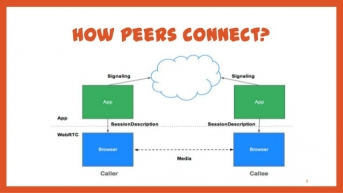
\includegraphics[width=0.8\linewidth]{peeeeer.jpg}
\caption{Why WebRTC}
\end{figure}

\end{block}

%----------------------------------------------------------------------------------------

\end{column} % End of column 2.1

\begin{column}{\onecolwid} % The second column within column 2 (column 2.2)

%----------------------------------------------------------------------------------------
%	RESULTS
%----------------------------------------------------------------------------------------

\begin{block}{Why WebRTC}

\begin{figure}
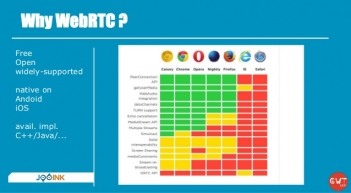
\includegraphics[width=0.8\linewidth]{why.jpg}
\caption{Why WebRTC}
\end{figure}


\begin{itemize}
\item WebRTC is open source so we don't have problems with privacy.
\item WebRTC improves connectivity and reduces data costs.
\item WebRTC improves latency and is simple to work with.
\item WebRTC guarantees high scalability and efficiency even for low bandwidth connections.
\end{itemize}



\end{block}

%----------------------------------------------------------------------------------------

\end{column} % End of column 2.2

\end{columns} % End of the split of column 2

\end{column} % End of the second column

\begin{column}{\sepwid}\end{column} % Empty spacer column

\begin{column}{\onecolwid} % The third column

\begin{figure}
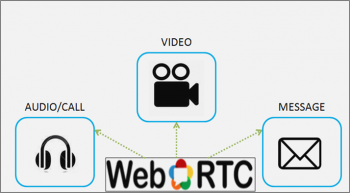
\includegraphics[width=0.8\linewidth]{whatt.png}
\caption{Why WebRTC}
\end{figure}


%----------------------------------------------------------------------------------------
%	CONCLUSION
%----------------------------------------------------------------------------------------

\begin{block}{Conclusion}

\begin{itemize}
\item Though there are existing systems like Skype and Hangouts, Ping guarentees around 60\% more efficiency.
\item Ping also guarentees high scalability. Around 3000 users per second.
\item As WebRTC is leveraging communication, Ping uses WebRTC to improved end user experience.
\end{itemize}

\end{block}

%----------------------------------------------------------------------------------------
%	ADDITIONAL INFORMATION
%----------------------------------------------------------------------------------------



%----------------------------------------------------------------------------------------
%	REFERENCES
%----------------------------------------------------------------------------------------

\begin{block}{References}

\begin{itemize}
\item https://webrtc.org
\item https://mozilla.org/webrtc
\item https://github.com/webrtc
\end{itemize}

\end{block}

%----------------------------------------------------------------------------------------
%	ACKNOWLEDGEMENTS
%----------------------------------------------------------------------------------------



%----------------------------------------------------------------------------------------
%	CONTACT INFORMATION
%----------------------------------------------------------------------------------------

\setbeamercolor{block alerted title}{fg=black,bg=norange} % Change the alert block title colors
\setbeamercolor{block alerted body}{fg=black,bg=white} % Change the alert block body colors

\begin{alertblock}{Contact Information}

\begin{itemize}
\item Web: \href{http://www.pingapp.xyz}{http://www.pingapp.xyz}
\end{itemize}
\item wasim@thabraze.me

\end{alertblock}


%----------------------------------------------------------------------------------------

\end{column} % End of the third column

\end{columns} % End of all the columns in the poster

\end{frame} % End of the enclosing frame

\end{document}

